%!TEX root = ../thesis.tex

\chapter{Dynamo Theory}
\label{chap:dynamotheory}
In its most basic form a dynamo is an engine which takes kinetic energy in the form of fluid motion and transforms it into magnetic energy. In many planetary cores this kinetic energy originates from thermal convection driven by the removal of heat from the core, however other sources of energy such as tidally \citep{cebron2014}, or precessionally driven flows \citep{tilgner2005} are possible. The physical mechanism by which this transfer from kinetic to magnetic energy occurs is summarised in the magnetic induction equation (section \ref{sec:magneticinduction}). 

\section{Maxwells Equations in Planetary Dynamos}
In order to see how dynamos turn fluid velocities into magnetic fields, we must first start with the basic laws concerning electricity and magnetism. The governing equations for this are Maxwell's equations:

\begin{equation}
\nabla \cdot \mbf{E}=\frac{\rho}{\epsilon_{o}}
\label{eq:gauss}
\end{equation}

\begin{equation}
\nabla \cdot \mbf{B}=0
\label{eq:monopoles}
\end{equation}

\begin{equation}
\nabla \times \mbf{B}=\mu_{o} \left(\mbf{J}+\epsilon_{o}\frac{\partial \mbf{E}}{\partial t}\right)
\label{eq:amperesfull}
\end{equation}

\begin{equation}
\nabla\times\mbf{E}=-\frac{\partial \mbf{B}}{\partial t}.
\label{eq:faraday}
\end{equation}
Where $\mbf{B}$ is the magnetic field, $\mbf{J}$ is the current density, $\mbf{E}$ is the electric field, $\rho$ is the charge density, $\epsilon_{o}$ is the electrical permittivity  of free space, and $\mu_{o}$ is the magnetic permeability of free space.

We also use Ohm's law, which relates electric fields to currents:
\begin{equation}
\mbf{J}=\sigma\mbf{E},
\label{eq:ohmslocal}
\end{equation}
where $\sigma$ is the electrical conductivity.

\subsection{The MHD Approximation}
We can approximate Maxwell's equations using the magnetohydrodynamic (MHD) approximation by considering the relative sizes of various terms. First we approximate equation \ref{eq:amperesfull} by comparing the terms $\nabla\times\mbf{B}$ and $\mu_{o}\epsilon_{o} \frac{\partial \mbf{E}}{\partial t}$:
\begin{equation}
\frac{\mu_{o}\epsilon_{o} \frac{\partial \mbf{E}}{\partial t}}{\nabla\times\mbf{B}}.
\end{equation}
Using Faraday's law (equation \ref{eq:faraday}) and characteristic scales for electric field, magnetic field, length and time ($E$, $B$, $L$ and $\tau$ respectively) we can scale $\mbf{E}\sim B L/\tau$ and using $\nabla\times\mbf{B}\sim B/L$ we get
\begin{equation}
\frac{\mu_{o} \epsilon_{o} L^2}{\tau^2}.
\end{equation}
If we take $\mbf{U}\sim L/\tau$ as a characteristic velocity and note that $1/\sqrt{\mu_{o}\epsilon_{o}}$ is the speed of light this becomes
\begin{equation}
\frac{\mu_{o}\epsilon_{o} \frac{\partial \mbf{E}}{\partial t}}{\nabla\times\mbf{B}}\sim\frac{U^2}{c^2}
\end{equation}
meaning the term $\mu_{o}\epsilon_{o} \frac{\partial \mbf{E}}{\partial t}$ is negligible for velocities much less than the speed of light. Since the characteristic velocity in planetary cores is $\mathcal{O}\left(10^{-4}\right) \textrm{m/s} \ll c$ we can safely discard this term in planetary dynamos giving 
\begin{equation}
\nabla \times \mbf{B}=\mu_{o}\mbf{J}.
\label{eq:amperes}
\end{equation}

Next we consider how fields transform between reference frames. We would like to frame our problem in the rotating reference frame of the planetary surface. However in a convecting system each parcel of fluid is moving with respect to the surface at any given time. This means that the quantities present in Maxwell's equations will vary for each parcel of fluid depending on the fluid's velocity with respect to the planetary surface reference frame. It is helpful to reformulate these equations in terms of the $\mbf{E}$, $\mbf{B}$, and $\mbf{J}$ fields that are measured in the planetary surface reference frame. We will denote the reference frame following the fluid as $A^\prime$, all quantities measured in that frame will be distinguished with primes as well. Quantities in the reference frame of the planetary surface will be unprimed. 

If we reformulate the Lorentz transformations in \citet{jackson1999} into components that are parallel ($\parallel$) and perpendicular ($\perp$) to the motion of the $A^\prime$ frame we get:
\begin{align}
\begin{split}
\mbf{E}_{\parallel}^\prime= {} & \mbf{E}_{\parallel}\\
\mbf{B}_{\parallel}^\prime= {} & \mbf{B}_{\parallel}\\
\mbf{J}_{\parallel}^\prime= {} & \gamma\left(\mbf{J}_{\parallel}-\rho\mbf{u}\right)\\
\end{split}
\begin{split}
\mbf{E}_{\perp}^\prime= {} & \gamma\left(\mbf{E}_{\perp}+\mbf{u}\times\mbf{B}_{\perp}\right)\\
\mbf{B}_{\perp}^\prime= {} & \gamma\left(\mbf{B}_{\perp}-\frac{1}{c^2}\mbf{u}\times\mbf{E}_{\perp}\right)\\
\mbf{J}_{\perp}^\prime= {} & \mbf{J}_{\perp}\\
\end{split}
\end{align}
where the velocity relative to the planetary surface frame is $\mbf{u}$ and 
\begin{align}
\gamma=\frac{1}{\sqrt{1-\frac{u^2}{c^2}}}.
\end{align}
For $u\ll c$ we can see that $\gamma\sim 1$. If we use the scaling $E\sim B U$ as before, and scale $\rho u\sim \epsilon_{o} \mu_{o} J L/\tau=J U/c^2$ (equations \ref{eq:faraday}, \ref{eq:gauss}, and \ref{eq:amperes}) these equations reduce to
\begin{align}
\mbf{E}^{\prime} = {} & \mbf{E}+\mbf{u}\times\mbf{B} \label{eq:lorentze} \\
\mbf{B}^{\prime} = {} & \mbf{B} \label{eq:lorentzb} \\
\mbf{J}^{\prime} = {} & \mbf{J} \label{eq:lorentzj}.
\end{align}
We now turn our attention to the Lorentz force. For a continuous charge distribution this is
\begin{equation}
\mbf{F}= \rho \mbf{E} + \mbf{J}\times\mbf{B}
\end{equation}
however using Maxwell's equations to scale $\mbf{E}$ as 
\begin{equation}
E\sim \frac{BL}{\tau} 
\label{eq:escale}
\end{equation}
and use equations \ref{eq:gauss}, \ref{eq:amperes}, and \ref{eq:escale} to show
\begin{align}
\frac{\rho \mbf{E}}{\mbf{J}\times\mbf{B}} = {} & \frac{\left| \epsilon_{0} \mbf{E} \nabla \cdot \mbf{E} \right|}{\left|\nabla\times\mbf{B} \times \mbf{B} /\mu_{o}\right|}\\
\sim {} & \epsilon_{0}\mu_{0} \frac{ E^{2} } { B^{2}  } \\
\sim {} & \frac{u^2}{c^2}\ll1
\end{align}
so the Lorentz force becomes $\mbf{F}=\mbf{J}\times\mbf{B}$.

The final equation we need to consider is Ohm's law (equation \ref{eq:ohmslocal}). This equation is valid for the reference frame of a fluid parcel, not for the planet centred reference frame in which we would like to frame our problem. In the notation of our Lorentz transformations Ohm's law would be written as 
\begin{equation}
\mbf{J}^\prime=\sigma \mbf{E}^{\prime}.
\end{equation}
We can very easily transform this to our planetary surface frame using the approximate Lorentz transformations we just described (equations \ref{eq:lorentze} and \ref{eq:lorentzj}):
\begin{equation}
\mbf{J}=\sigma \left(\mbf{E}+\mbf{u}\times\mbf{B}\right).
\label{eq:ohms}
\end{equation}

\section{Magnetic Induction}
\label{sec:magneticinduction}
In order to see how the transfer of mechanical to magnetic energy occurs we start with Faraday's  law, Amp\`eres law,  and Ohm's law (equations \ref{eq:faraday}, \ref{eq:amperes} and \ref{eq:ohms} respectively). We can put these equations into a more intuitive and convenient form by some simple vector calculus. Taking the curl of Ohm's law (equation \ref{eq:ohms}):
\begin{equation}
\nabla\times\mbf{J}=\sigma \left(\nabla\times\mbf{E}+\nabla\times\left(\mbf{u}\times\mbf{B}\right)\right).
\end{equation}
If we substitute $\mbf{J}$ from equation \ref{eq:amperes} and $\nabla\times\mbf{E}$ from equation \ref{eq:faraday} and rearrange slightly this becomes
\begin{equation}
\frac{\partial \mbf{B}}{\partial t}=\nabla\times\left(\mbf{u}\times\mbf{B}\right)-\frac{1}{\mu_o \sigma}\nabla\times\nabla\times\mbf{B}.
\end{equation}
We can then use the vector identity $\nabla\times\nabla\times\mbf{B}=\nabla\left(\nabla\cdot\mbf{B}\right) -\nabla^{2}\mbf{B}$ along with the fact that magnetic fields are divergenceless to get the magnetic induction equation:
\begin{equation}
\label{eq:dimensionalmagnetic}
\frac{\partial \mbf{B}}{\partial t} = \nabla\times\left(\mbf{u}\times\mbf{B}\right) +\eta \nabla^{2}\mbf{B},
\end{equation}
here we have introduced a quantity known as the magnetic diffusivity ($\eta=1/\sigma \mu_{o}$). This equation relates fluid velocities ($\mbf{u}$) and magnetic fields ($\mbf{B}$) to the time rate of change of the magnetic field. This provides a mechanism by which a planet can  generate a magnetic field. 

%The toroidal and poloidal decomposition we discussed earlier becomes particularly useful now because of the form of equation \ref{eq:dimensionalmagnetic}. If we decompose this equation with the toroidal-poloidal expansion in spherical coordinates to write two scalar evolution equations, we find that the linear parts (the time derivative and the diffusive term) of the equations are independent of each other, and that the only coupling between them is in the inductive term.

\subsection{Interpreting the Magnetic Induction Equation}
\subsubsection{Frozen Flux Theorem and Connections to Fluid Mechanics}
\label{sec:frozenflux}
While the details of the magnetic induction equation (equation \ref{eq:dimensionalmagnetic}) are somewhat opaque, its terms can be interpreted relatively easily. On the right hand side the term $\eta \nabla^{2} \mbf{B}$ is a diffusive term, indicating that magnetic field can diffuse away via ohmic dissipation. The other term, $\nabla\times\left(\mbf{u}\times\mbf{B}\right)$, is less straightforward, but clearly represents interactions between the velocity and magnetic fields. In order for the magnetic field to grow in time, this must be a generation term which is larger than the diffusive term. The relative size of magnetic field generation to diffusion  can be approximately quantified by the magnetic Reynolds number ($\textrm{Re}_{M}$), which is a non-dimensional number found by taking the ratio of these two terms:
\begin{equation}
\textrm{Re}_{M}= \frac{\nabla\times\left(\mbf{u}\times\mbf{B}\right)}{\eta \nabla^{2}\mbf{B}}\sim \frac{UL}{\eta}.
\end{equation}
While it may seem intuitive that $\textrm{Re}_{M}> 1$ should result in magnetic field growth in excess of diffusion, the largest known theoretical lower bound for magnetic field generation is $\textrm{Re}_{M}\sim10$ \citep{BackusBound,ProctorBound}. This is a necessary, but not sufficient condition for magnetic field generation. In numerical dynamo models, magnetic Reynolds numbers on the order of 40 are typical lower bounds  \citep{OlsonandChristensen2006}.

Some intuition about how the magnetic induction equation behaves comes from using the vector identity $\nabla\times\left(\mbf{A}\times\mbf{B}\right)=\mbf{A}\left(\nabla\cdot\mbf{B}\right)-\mbf{B}\left(\nabla\cdot\mbf{A}\right)+\left(\mbf{B}\cdot\nabla\right)\mbf{A}-\left(\mbf{A}\cdot\nabla\right)\mbf{B}$, the divergenceless property of magnetic fields  ($\nabla \cdot \mbf{B}=0$) and by assuming fluid incompressibility\footnote{$\nabla\cdot\mbf{u}=0$, see section \ref{sec:fluidflow} for more information on this approximation.}. With appropriate manipulation equation \ref{eq:dimensionalmagnetic} becomes
\begin{equation}
\frac{\partial \mbf{B}}{\partial t} +\mbf{u}\cdot\nabla\mbf{B}=\mbf{B}\cdot\nabla \mbf{u}+\eta\nabla^{2}\mbf{B}.
\end{equation}
In the limit of infinite electrical conductivity (or zero magnetic diffusivity) this equation becomes
\begin{align}
\frac{\partial \mbf{B}}{\partial t} +\mbf{u}\cdot\nabla\mbf{B}= & {} \mbf{B}\cdot\nabla \mbf{u}\\
\frac{D \mbf{B}}{D t}=& {}\mbf{B}\cdot\nabla \mbf{u}
\label{eq:mievort}
\end{align}
where $D/Dt$ is the advective derivative of fluid mechanics. This equation has the same form as the well known baratropic vorticity equation of atmospheric dynamics. A consequence of that equation is that the vorticity is frozen into the fluid \citep{Vallis}. This is also true of magnetic fields in the magnetic induction equation with an infinite electrical conductivity (zero magnetic diffusivity). In magnetohydrodynamics, this is widely known as the ``frozen flux'' theorem.

We can expand one component (we will choose the $x$ component) of equation \ref{eq:mievort} to get
\begin{equation}
\frac{D B_{x}}{Dt}=B_{x}\frac{\partial u_{x}}{\partial x}+B_{y}\frac{\partial u_{x}}{\partial y}+B_{z}\frac{\partial u_{x}}{\partial z}.
\end{equation}
We can interpret each of these terms as either stretching or tilting magnetic field. The second and third are ``tilting'' terms that tell us that we can increase the magnetic field strength in the $x$-direction by re-orienting magnetic field that is in the $y$- or $z$-directions as long as $u_x$ varies in those directions. The first term is the ``stretching'' term in the magnetic induction equation. This tells us that  spatial gradients of $u_x$ in the $x$-direction can stretch the component of the magnetic field which is co-linear with the velocity. 

\section{Fluid Flow in Planetary Cores}
\label{sec:fluidflow}
The flows in planetary cores are governed by the Navier-Stokes equation modified with the appropriate forces. In its most general form this is
\begin{equation}
\rho\left(\frac{\partial}{\partial t}+\mbf{u}\cdot\nabla\right)\mbf{u}=-\nabla p +\nabla\cdot\mbf{T}+\mbf{F},
\label{eq:navierstokesgeneral}
\end{equation}
here $\rho$ is the fluid density, $p$ is the pressure gradient, $\mbf{T}$ is the deviatoric stress tensor representing shear forces, and $\mbf{F}$ represents body forces.

In the Earth's core there are three body forces which are generally used in geodynamo models. These include the Coriolis and Lorentz forces which represent the apparent force of rotation and  magnetic fields respectively, as well as the gravitational force, which allows free convection to occur. Adding these to equation \ref{eq:navierstokesgeneral} gives
\begin{equation}
\rho\left(\frac{\partial}{\partial t}+\mbf{u}\cdot\nabla\right)\mbf{u}+2\rho\mbf{\Omega}\times\mbf{u}=-\nabla p +\mbf{J}\times\mbf{B}+\rho \mbf{g}+\nabla\cdot\mbf{T}
\label{eq:navierstokesgeneralcorlor}
\end{equation}
where $\mathbf{g}$ is the acceleration due to gravity and $\mbf{\Omega}$ is the planetary rotation vector. This equation can be closed by the addition of a conservation of mass equation:
\begin{equation}
\frac{\partial \rho}{\partial t}=\nabla\cdot\left(\rho \mbf{u}\right).
\label{eq:conservationofmass}
\end{equation}
The liquid in the cores of terrestrial planets is mostly iron which is relatively incompressible. To simplify these equations we make use of one of the simplifications involved in the the Boussinesq approximation, that density variations can be neglected except when they multiply the acceleration due to gravity. Under this approximation, equation \ref{eq:conservationofmass} becomes
\begin{equation}
\nabla\cdot\mathbf{u}=0.
\end{equation}
If we finally assume that the fluid is Newtonian we can represent equation \ref{eq:navierstokesgeneralcorlor} as
\begin{equation}
\rho_{o}\left(\frac{\partial}{\partial t}+\mbf{u}\cdot\nabla\right)\mbf{u}+2\rho_{o}\mbf{\Omega}\times\mbf{u}=-\nabla p +\mbf{J}\times\mbf{B}+\Delta\rho \mbf{g}+\rho_{0}\nu\nabla^{2}\mbf{u}.
\label{eq:dimensionalmomentumgeneralbuoyancy}
\end{equation}
In this equation $\rho_{o}$ is the average fluid density, $\nu$ is the kinematic viscosity, and $\Delta\rho$ is the departure from the average density due to thermal or compositional variations.
\subsection{Interpreting the Momentum Equation}
We can gain some insight into how the momentum equation  behaves by considering different force balances. This involves assuming that various terms in equation \ref{eq:dimensionalmomentumgeneralbuoyancy} balance each other exactly, neglecting all other forces. While this is a crude approximation, it allows us to gain some insight into the general behaviour of dynamos.

\subsection{Geostrophic Balance}
If we neglect magnetic fields temporarily and furthermore assume that viscosity, buoyancy and fluid inertia are small, we get a force balance between the pressure gradient and the Coriolis force:
\begin{equation}
\label{eq:geostrophicbalance}
2\rho_{o}\mbf{\Omega}\times\mbf{u}=-\nabla p.
\end{equation}
Taking the the curl of both sides, and using the incompressibility of our fluid gives
\begin{equation}
\pderiv[1]{\mbf{u}}{z}=0 \label{eq:taylorproudman},
\end{equation}
where we take $\hat{z}$ as a unit vector aligned with the axis of rotation. This result is known as the Taylor-Proudman theorem  \citep{proudman1916,taylor1917} and it implies that the fluid motion is invariant along the axis of rotation telling us that convection in rapidly rotating planets should take on a columnar structure with columns aligned along the rotation axis. A representation of this is shown in figure \ref{fig:rolls}.
\begin{figure}
	\centering
	\noindent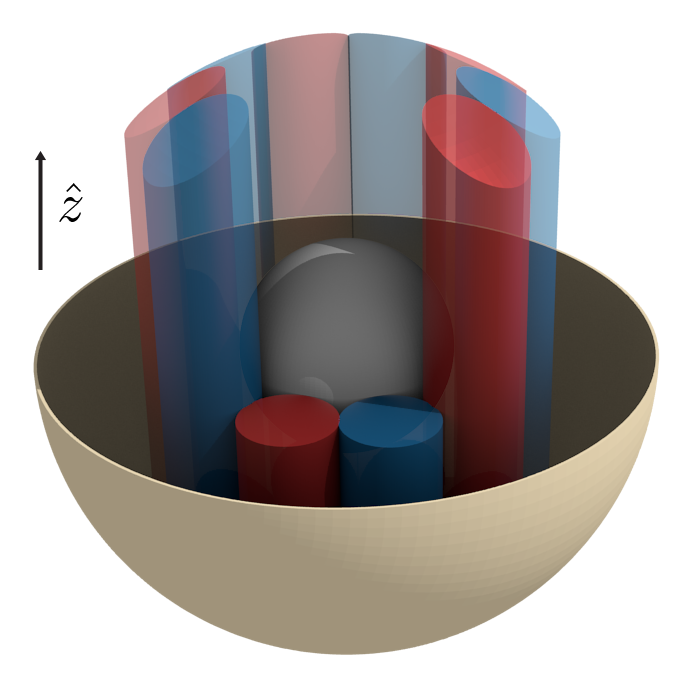
\includegraphics[width=.65\linewidth]{Chapter2/figures/Rolls.png}
	\caption{Convection rolls in an Earth-like core. Red rolls indicate clockwise fluid motion and blue rolls indicate counterclockwise fluid motion. The fluid velocities are invariant along the axis of rotation ($\hat{z}$) due to the Taylor-Proudman theorem. Here the yellow half-sphere is a cutaway of the core-mantle boundary and the grey inner sphere represents the inner core boundary.}
	\label{fig:rolls}
\end{figure}

\subsection{Magnetostrophic Balance}
\label{subsec:magnetostrophic}
If we add magnetic fields to equation \ref{eq:geostrophicbalance} and assume that the Lorentz force balances the Coriolis force and the pressure gradient we get a different expression
\begin{equation}
2\rho_{o}\mbf{\Omega}\times\mbf{u}=-\nabla p + \mbf{J}\times\mbf{B}.
\end{equation}
If we compare the relative strengths of the Coriolis and Lorentz forces we can derive a non-dimensional number known as the Elsasser number 
\begin{align}
\Gamma =& {} \frac{ \mbf{J}\times\mbf{B}}{2\rho_{o}\mbf{\Omega}\times\mbf{u}}\\
 \approx & {} \frac{B^{2}}{2\Omega \eta \rho \mu_{o} }
\end{align}
where $B$ represents a characteristic magnetic field strength and we have taken the magnetic diffusion time ($L^{2}/\eta$) as our characteristic timescale.

This balance is important because if we assume an Elsasser number we can get an estimate of magnetic field strength in the core. An Elsasser number of $\mathcal{O}\left(1\right)$ is a common balance to use, implying all forces besides the Coriolis and Lorentz forces are negligible, and results in a magnetic field strength estimate of $B\approx\sqrt{2\Omega \eta \rho \mu_{o}}$. This balance is called magnetostrophic balance and dynamos which display this are known as strong field dynamos.

\section{Thermal Equation}
The buoyancy force in the momentum equation enters as $\Delta\rho \mbf{g}$ and represents any buoyancy due to compositional or thermal effects. In the planetary dynamo community it is common to combine the effects of temperature and composition into a single variable known as co-density. As they are both important effects in the core, ideally the dynamics of composition and temperature should be solved separately. Each have characteristic diffusivities, which differ by three orders of magnitude \citep{Braginsky1995}, the thermal diffusivity being greater than the compositional diffusivity. In this thesis we adopt the common practice of assuming that small scale (and unresolved) turbulence is present, this acts on both quantities equally and results in an effective turbulent diffusivity which is the same for all quantities. This allows us to introduce the co-density $C$, which is a mixture of compositional and thermal differences with a common  diffusivity due to unresolved turbulence \citep{Braginsky1995, wicht2008}.

The evolution of co-density in the Boussinesq approximation is governed by an energy equation: 
\begin{equation}
\pderiv[1]{C}{t}+\left(\mbf{u}\cdot\nabla\right)C=\kappa \nabla^{2} C + Q\left(r\right).
\label{eq:fullcodensity}
\end{equation}
Here $\kappa$ is the co-density diffusivity and $Q$ represents any co-density sources or sinks within the fluid region. If it is taken to be constant it often corresponds to a volumetric heat source such as radioactivity, or the evolution of the core's composition due to light element release in compositional convection.
 
We find it convenient to break up the co-density variable into a radially symmetric background state ($C_{o}$) and a perturbation ($\Theta$) which contains the dynamics of the co-density:
\begin{equation}
C=C_{o}\left(r\right)+\Theta\left(\mbf{r},t\right).
\end{equation}
Substituting this definition into equation \ref{eq:fullcodensity} gives
%\frac{\partial C_{o}}{\partial t}+\frac{\partial \Theta}{\partial t}+\left(\mbf{u}\cdot\nabla\right)C_{o}+\left(\mbf{u}\cdot\nabla\right)\Theta=\kappa\nabla^{2}C_{o}+\kappa\nabla^{2}\Theta +Q\left(r\right)
\begin{equation}
\pderiv[1]{C_{o}}{t}+\pderiv[1]{\Theta}{t}+\left(\mbf{u}\cdot\nabla\right)C_{o}+\left(\mbf{u}\cdot\nabla\right)\Theta=\kappa\nabla^{2}C_{o}+\kappa\nabla^{2}\Theta +Q\left(r\right)
\end{equation}
This equation can be separated into two equations, one of which involves only $C_{o}$ and $Q$, while the other contains $\Theta$ and $\mbf{u}$:
\begin{equation}
\pderiv[1]{\Theta}{t}+\left(\mbf{u}\cdot\nabla\right)\left(\Theta+C_{o}\left(r\right)\right)=\kappa \nabla^{2} \Theta\label{eq:dimensionalcodensity}
\end{equation}
\begin{equation}
\kappa\nabla^{2}C_{o}\left(r\right)=-Q\left(r\right).
\label{eq:dimensionalbgcodensity}
\end{equation}
Here equation \ref{eq:dimensionalcodensity} corresponds to the evolution equation for the co-density perturbation and equation \ref{eq:dimensionalbgcodensity} corresponds to the ODE defining the background co-density state. This formalism has a number of advantages, chief among which is that the background state can satisfy the non-homogeneous boundary conditions this problem poses, leaving the evolution equation with relatively simple boundary conditions.

\subsection{Co-Density in the Momentum Equation}
This definition of co-density influences our interpretation of the buoyancy term in the momentum equation. It becomes:
\begin{equation}
\Delta\rho \mbf{g} = \alpha g C \mbf{r},
\label{eq:dimmombuoyancy}
\end{equation}
where $\alpha$ is the co-density expansion coefficient and $\mbf{r}$ is a radial position vector. This assumes that the gravitational acceleration in a planetary core is directed radially and varies linearly with radius (a result easily derivable from Gauss's law). Substituting our definition of co-density into equation \ref{eq:dimensionalmomentumgeneralbuoyancy} gives:
\begin{equation}
\rho_{o}\left(\frac{\partial}{\partial t}+\mbf{u}\cdot\nabla\right)\mbf{u}+2\rho_{o}\mbf{\Omega}\times\mbf{u}=-\nabla p +\mbf{J}\times\mbf{B}+\alpha g r C_{o}\left(r\right)\mbf{\hat{r}}+\alpha g r \Theta\left(\mbf{r},t\right)\mbf{\hat{r}}+\rho_{o}\nu\nabla^{2}\mbf{u}.
\end{equation}
We can then define a modified pressure $\widetilde{p}$ such that
\begin{equation}
\nabla\widetilde{p}=\nabla p-\alpha g r C_{o}\left(r\right)\mbf{\hat{r}}
\end{equation}
which simplifies our momentum equation to
\begin{equation}
\rho_{o}\left(\frac{\partial}{\partial t}+\mbf{u}\cdot\nabla\right)\mbf{u}+2\rho_{o}\mbf{\Omega}\times\mbf{u}=-\nabla \widetilde{p} +\mbf{J}\times\mbf{B}+\alpha g r \Theta\mbf{\hat{r}}+\rho_{o}\nu\nabla^{2}\mbf{u}.
\label{eq:dimensionalmomentum}
\end{equation}
\section{Non-Dimensionalization}
\begin{figure}
	\centering
	\noindent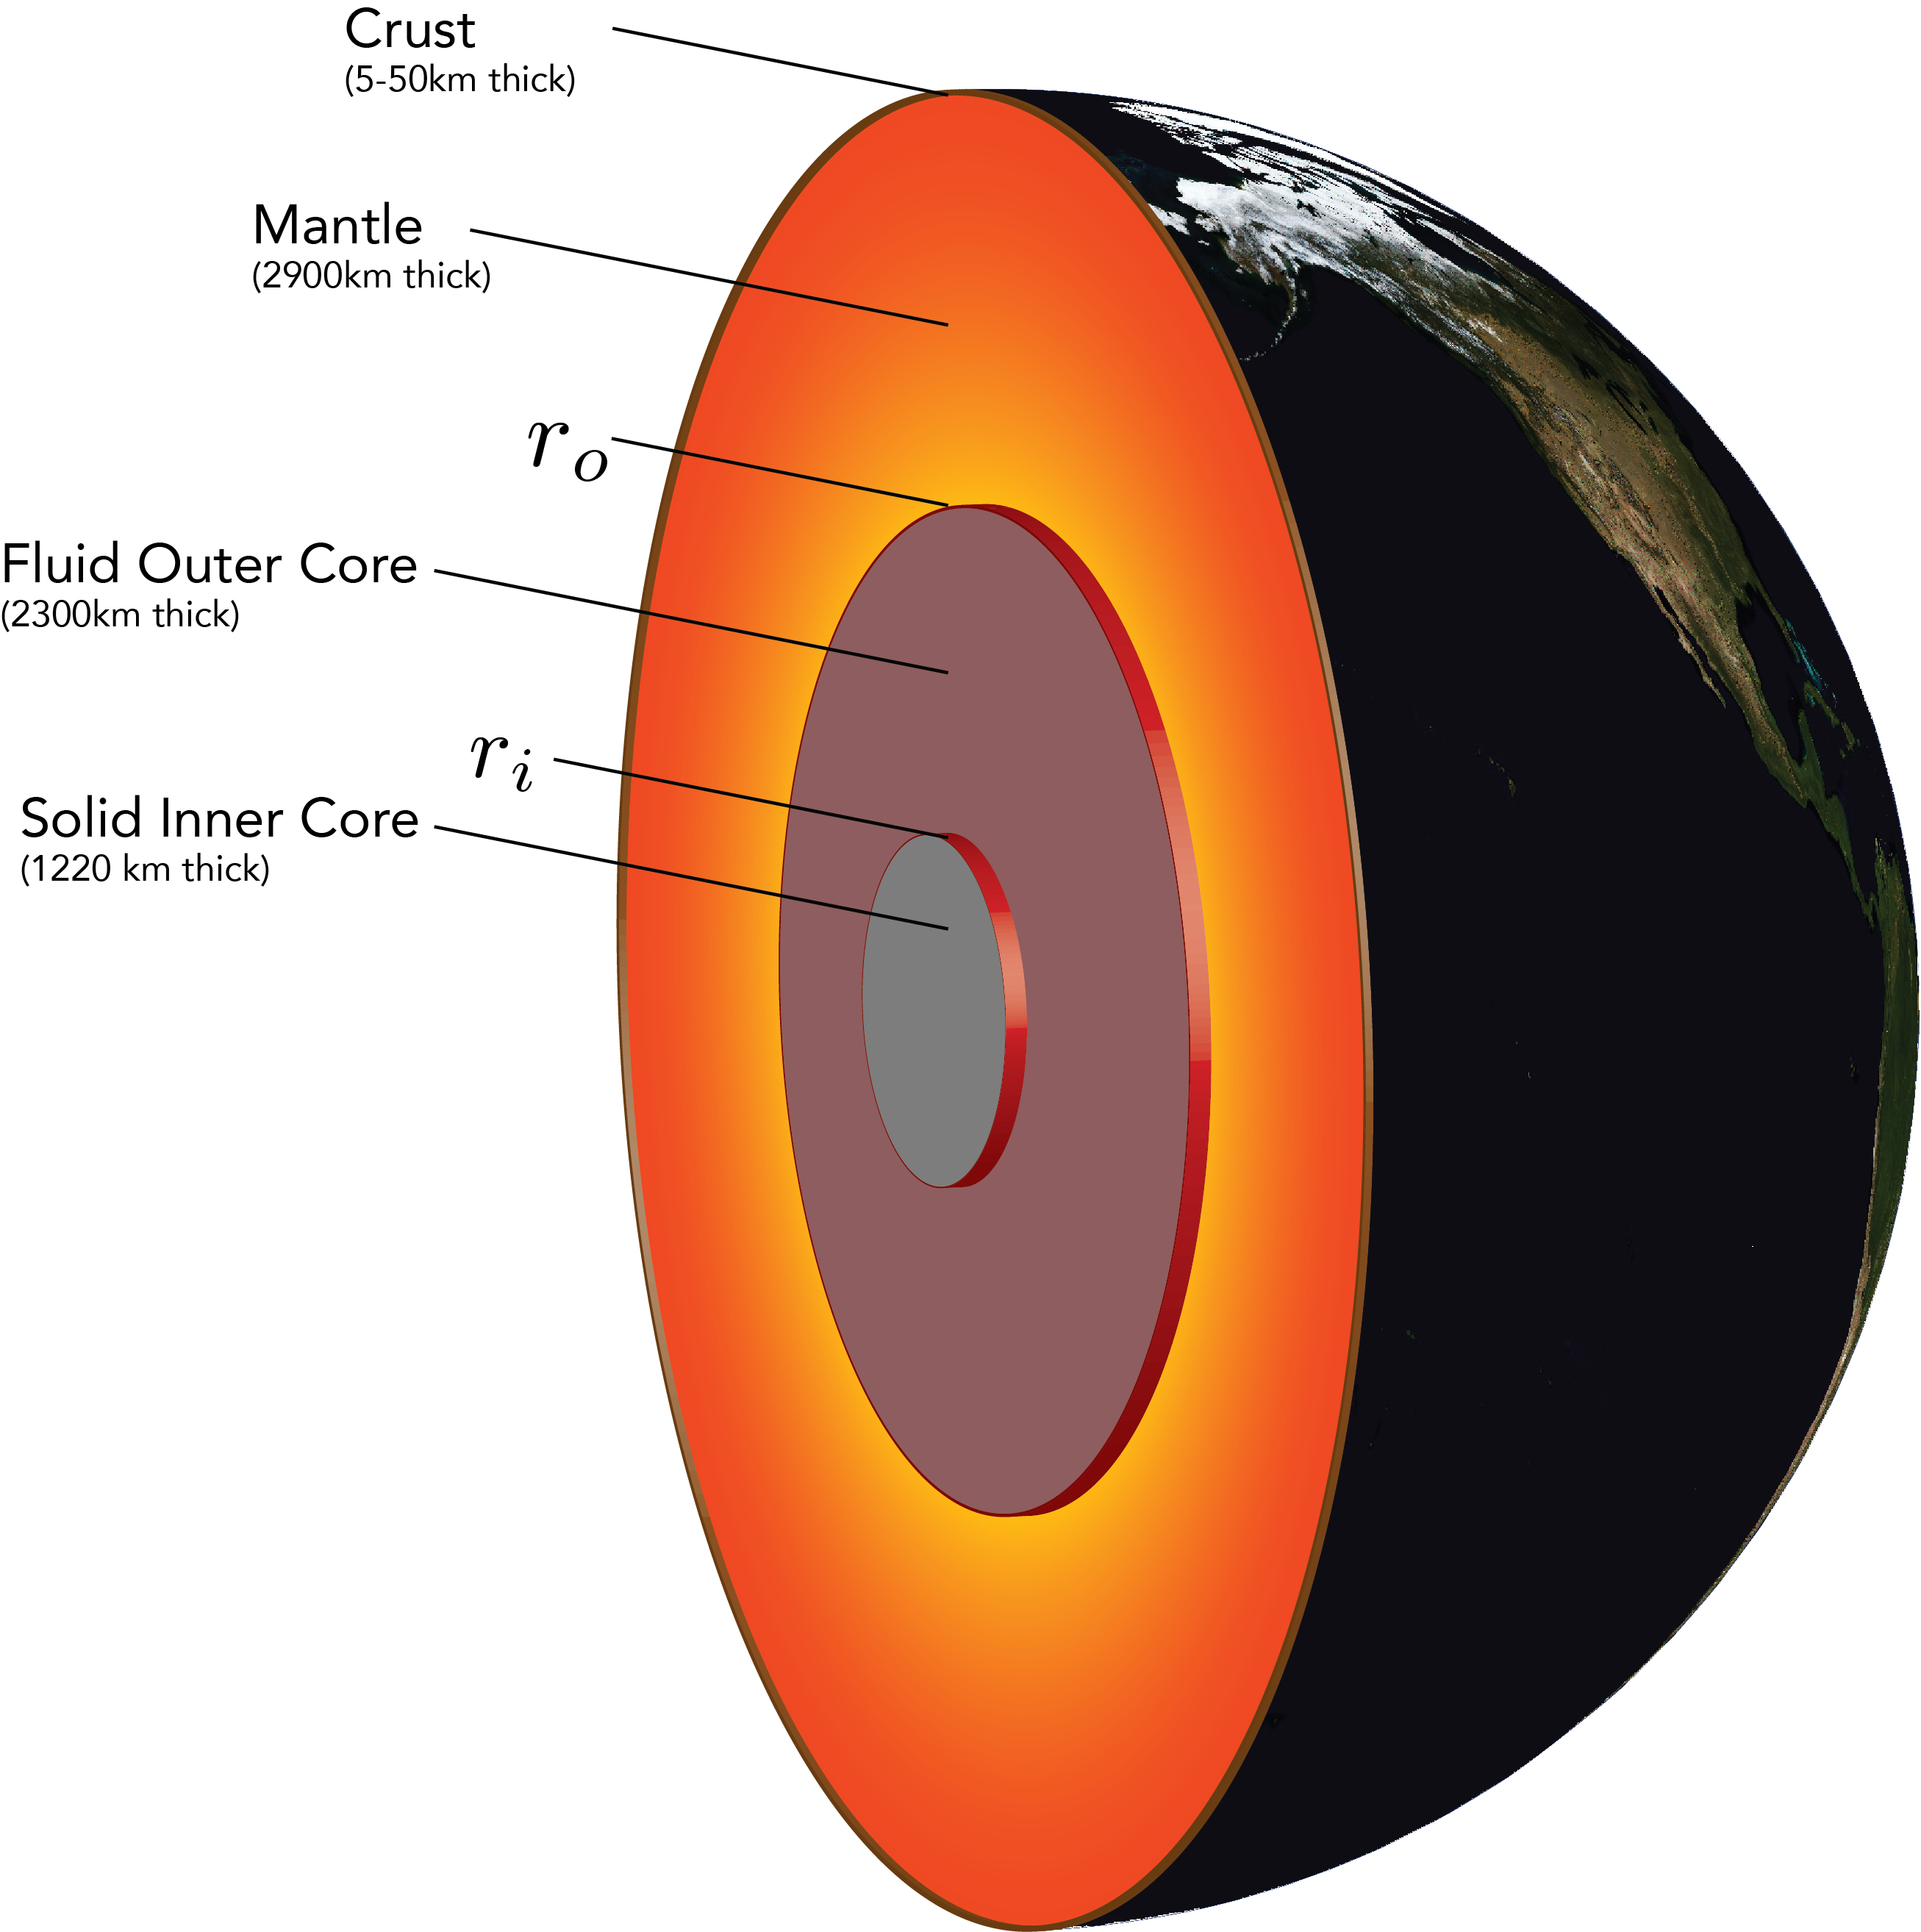
\includegraphics[width=.6\linewidth]{Chapter2/figures/CutawayEarth.png}
	\caption{A cutaway view of the structure of the Earth.}
	\label{fig:CutawayEarth}
\end{figure}
We wish to solve the momentum and co-density equations (equations \ref{eq:dimensionalcodensity}, \ref{eq:dimensionalbgcodensity}, and \ref{eq:dimensionalmomentum} ) in a spherical shell. This corresponds to the core of a planet with a solid inner core of radius $r_i$, and a rigid upper boundary of radius $r_o$ (see figure \ref{fig:CutawayEarth}). 

If we are to non-dimensionalise our equations we would like to pick units which have a physical relevance to the problem we wish to solve. For this reason we choose the outer core radius ($r_{o}$) as our length scale and choose the magnetic diffusion time $\tau=r_{o}^{2}/\eta$ as our timescale. To get a scale for the magnetic field, we follow the method outlined in section \ref{subsec:magnetostrophic} and assume an Elsasser number of 1, giving $B=\sqrt{2\Omega\eta\rho\mu_{o}}$. Finally we choose $h_{C} r_o$ as our co-density scale where $h_{C}$ is the co-density flux at the inner core boundary.

When we apply these non-dimensionalisations, equations \ref{eq:dimensionalmagnetic}, \ref{eq:dimensionalcodensity}, \ref{eq:dimensionalbgcodensity}, and \ref{eq:dimensionalmomentum} become
\begin{align}
Ro\left(\frac{\partial}{\partial t}+\mbf{u}\cdot\nabla\right)\mbf{u}+\mbf{\hat{z}}\times\mbf{u}=& {} -\nabla p+\mbf{J}\times\mbf{B}+Ra\Theta\mbf{r}+E\nabla^{2}\mbf{u} \label{eq:nondimmomentum}\\
\frac{\partial \Theta}{\partial t}+\mbf{u}\cdot\nabla C =& {}q_{\kappa}\nabla^{2}\Theta \label{eq:nondimcodensity}\\
\frac{\partial \mbf{B}}{\partial t}=& {} \nabla\times\left(\mbf{u}\times\mbf{B}\right)\label{eq:nondimmagnetic}+\nabla^{2}\mbf{B}.
\end{align}
The nondimensional parameters in equations (\ref{eq:nondimmomentum}) to (\ref{eq:nondimmagnetic}) are the Rayleigh number ($Ra$), the magnetic Rossby number ($Ro$), the magnetic Prandtl number ($q_{\kappa}$), and the Ekman number ($E$). These are given by:
\begin{align}
Ra=& {}\frac{\alpha g_{o}h_{C}r_{o}^{2}}{2\Omega\eta} \label{eq:rayleigh}\\
Ro=& {}\frac{\eta}{2\Omega r_{o}^{2}}\\
q_{k}=& {}\frac{\kappa}{\eta}\\
E=& {}\frac{\nu}{2\Omega r_{o}^2} \label{eq:ekman}.
\end{align}
The Rayleigh number defined in equation \ref{eq:rayleigh} is a modified Rayleigh number that differs in form from the Rayleigh number used in mantle convection. In non-rotating convection it is useful to define the Rayleigh number as the ratio between buoyancy and viscous forces, as viscosity is often the force that buoyancy must overcome in order for convection to occur. In rotating core convection, viscosity is typically very small, and buoyancy must overcome the ``stiffness'' of the fluid imposed by Taylor-Proudman theorem (equation \ref{eq:taylorproudman}) in order for convection to occur. For this reason we define the Rayliegh number as the ratio between the buoyancy force and the Coriolis force. As the Ekman number (equation \ref{eq:ekman}) is the ratio of the viscous force to the Coriolis force, a more conventional Rayleigh number can be recovered by dividing the modified Rayleigh number by the Ekman number.


\section{The Local Rossby Number}
\label{sec:rol}
One factor which makes dynamos difficult to understand is the large number of control parameters that are required to specify a solution to the governing equations. This is particularly troubling because the properties of a dynamo are dependent on the values of these control parameters. Unfortunately, for numerical reasons, dynamo models must be run in a parameter regime for which most of the control parameters are not appropriate for modelling planetary cores.

\citet{christensen06scaling} developed a scaling law concerning planetary dynamos which has proved to be useful in the prediction of the bulk properties of a dynamo as a function of its control parameters. The Rossby number is normally defined as the ratio of the inertial force to the Coriolis force, from equation \ref{eq:navierstokesgeneralcorlor} this is
\begin{align*}
Ro&=\frac{\left|\rho \mbf{u}\cdot\nabla\mbf{u}\right|}{\left|2\rho\mbf{\Omega}\times\mbf{u}\right|}\\
&\approx\frac{U}{\Omega r_o}.
\end{align*}
\citet{christensen06scaling} noted that while the inertial term depends on the length scale of the flow, the Coriolis term does not. They posited that a better measure of the role rotation plays in a given flow may be a Rossby number which depends on the characteristic length scale of the flow, rather than the characteristic length scale of the container. They defined this length scale as
\begin{equation}
\label{eq:rollength}
\bar{\ell}_{u}=\frac{4Ro_m^2}{\left(1-r_{io}\right)^2}\frac{\sum l\left\langle\mbf{u}_{l}\cdot\mbf{u}_{l}\right\rangle}{2E_{kin}}
\end{equation}
where $E_{kin}$ is the kinetic energy, defined as
\begin{equation}
E_{kin}=\frac{4 Ro_m^2}{\left(1-r_{io}\right)^{5}}\frac{1}{2}\int_{V}\left(\mbf{u}\cdot\mbf{u}\right)dV
\end{equation}
using the non-dimensionalisation of \citet{kuangandbloxham1999}. The factor in front of the integral results from converting the non-dimensionalisation from those used in \citet{christensen06scaling}. Combining these we get
\begin{equation}
\bar{\ell}_{u}=\left(1-r_{io}\right)^{3}\frac{\sum l\left\langle\mbf{u}_{l}\cdot\mbf{u}_{l}\right\rangle}{\int_{V}\left(\mbf{u}\cdot\mbf{u}\right)dV}.
\end{equation}
Since the mean radius to a point inside the shell is of order one, they set the half wavelength of the flow to $\pi/\ell_u$ giving a local Rossby number of 
\begin{equation}
\label{eq:rol}
Ro_{l}=Ro\frac{\bar{\ell}_{u}}{\pi}.
\end{equation}

\citet{christensen06scaling} then noted that the dipole dominance of the poloidal magnetic field depended strongly on the local Rossby number. They showed that dynamo models which had $Ro_{l}\leq 0.12$ had magnetic fields that were predominantly dipolar, while models with $Ro_{l}>0.12$ generated multipolar magnetic fields. This sharp transition is clear if the dipole dominance of the observable magnetic field ($f_{dip}$) is plotted against the local Rossby number (figure \ref{fig:rolfdip}). Using angle brackets to denote a time average, $f_{dip}$ is defined as
\begin{equation}
f_{dip}=\left\langle\frac{ \int_S \sqrt{\mbf{B}_{l=1}\cdot\mbf{B}_{l=1}} }{\sum_{l=1}^{12} \int_S  \sqrt{\mbf{B}_{l}\cdot\mbf{B}_{l}}}\biggr\rvert_{r=r_{o}}\right\rangle
\end{equation}
which is the time average ratio of the r.m.s. amplitude of the dipole field to the r.m.s. amplitude of the field in the first 12 degrees.
\begin{figure}
	\centering
	\noindent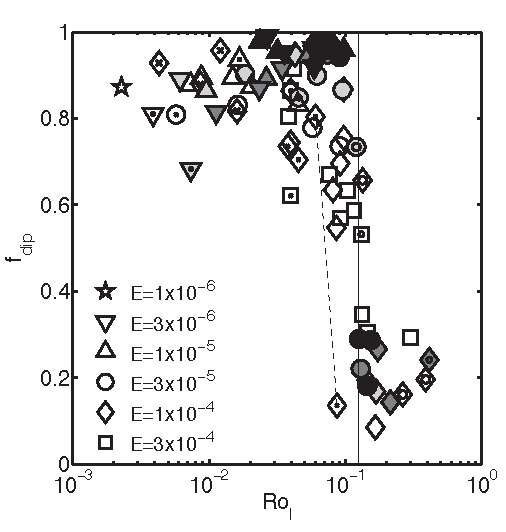
\includegraphics[width=.5\linewidth]{Chapter2/figures/fdip.pdf}
	\caption{The dipole dominance ($f_{dip}$) of the observable magnetic field as a function of the local Rossby number. Here $f_{dip}$ is defined as the time average ratio of the r.m.s. amplitude of the dipole field to the r.m.s. amplitude of the field in the first 12 degrees. The Ekman numbers here are in the variables of \citet{christensen06scaling}, they can be converted to the Ekman numbers in this work by multiplying them by a factor of $0.21125$. This figure is reproduced from \citet{christensen06scaling} where it is figure 3.}
	\label{fig:rolfdip}
\end{figure}

Once the local Rossby number is defined, a natural extension is to apply it to the planets of our solar system. The definition of equation \ref{eq:rol} requires a knowledge the characteristic fluid velocity and scale in the fluid outer core. This is very unconstrained for even the Earth, and less well constrained for other planets of our solar system. An alternative approach is to construct scaling laws which relate the control parameters of the dynamo to the local Rossby number. The control parameters depend on the physical properties of the planet (e.g. diffusivities, rotation rates etc.) which are known more accurately than the dynamical properties (i.e. the scale of convection).

Several studies have constructed scaling laws which relate the dynamo control parameters to the local Rossby number \citep{christensen06scaling,OlsonandChristensen2006,aubert2009}. The most general is from \citet{aubert2009}, if it is cast into the non-dimensionalisation used in this work it can be written as
\begin{equation}
Ro_{l}=0.674\frac{1+r_{io}}{\left(1-r_{io}\right)^{-0.64}}p^{0.48}E^{-0.32}q_{\kappa}^{-0.19}.
\label{eq:rolscaling}
\end{equation}
$p$ is the convective power density. Assuming the background state does not change the convective power density can be written as
\begin{equation}
p=\frac{3}{2}\frac{(1-r_{io})^2}{\left(1-r_{io}^3\right)} \left[(1-f_{i})\left(\frac{1}{(1-r_{io})^2}-\frac{3}{5}\frac{\left(1-r_{io}^5\right)}{\left(1-r_{io}^3\right)}\right)+f_{i} \left(\frac{3}{5}\frac{\left(1-r_{io}^5\right)}{\left(1-r_{io}^3\right)}-\frac{r_{io}^2}{(1-r_{io})^2}\right)\right]Ra_Q
\end{equation}
where $f_i$ is the fraction of the total buoyancy flux injected at the inner core and $Ra_Q$ is a Rayleigh number based on advected buoyancy flux \citep{aubert2009}.

\section{Magnetic Screening by Conductors}
\label{sec:screeningderiv}
Two projects within this thesis will involve the effect of a solid conducting layer placed between the dynamo region and the planetary surface. It is therefore worthwhile to discuss the effect of this layer on the observable magnetic field. In the absence of fluid motion, the magnetic induction equation (equation \ref{eq:dimensionalmagnetic}) becomes a diffusion equation:
\begin{equation}
\pderiv[1]{\mbf{B}}{t}=\eta\nabla^{2}\mbf{B}.
\end{equation}
To illustrate the screening effect we will solve this equation in a cartesian geometry with a constant diffusivity. We will solve this system in a semi-infinite ($z>0$), cartesian geometry, and apply a magnetic field that oscillates with frequency $\omega$ at the finite boundary. In this geometry, this system is described as
\begin{align}
\pderiv[1]{B}{t}= & {}\eta\pderiv[1]{B}{z} \label{eq:conlayerdiffusion} \\
B\left(z=0,t\right)= & {}\sin\left(\omega t\right) \\
B\left(z \to \infty,t\right)= & {} 0
\end{align}
Where $B$ is an arbitrary component of $\mbf{B}$. An ansatz of the form
\begin{equation}
B=B_{0}e^{-\gamma z} \sin\left(kz-\omega t\right)
\label{eq:bansatz}
\end{equation}
satisfies the boundary conditions and implies a wave-like solution that decays to infinity. Substituting equation \ref{eq:bansatz} into equation \ref{eq:conlayerdiffusion} we find  
\begin{equation}
-B_{0}\omega  e^{-\gamma  z} \cos (k z-\omega t  )=\eta B_{0} e^{-\gamma  z} \left[\left(\gamma ^2-k^2\right) \sin (k z- \omega t
    )-2 \gamma  k \cos (k z- \omega t  )\right].
\end{equation}
This implies that a solution requires $\gamma=\pm k, k=\sqrt{\pm \omega / 2 \eta}$. Here we pick the branch which leads to physicsl (real) solutions and finite solutions at infinity. Equation \ref{eq:bansatz} becomes
\begin{equation}
B=B_{0}e^{-\sqrt{\omega/\left(2\eta\right)} z} \sin\left(\sqrt{\frac{\omega}{2\eta}}z-\omega t\right)
\end{equation}
Recasting $\omega$ from a frequency to a timescale ($\tau \sim 1/\omega$) this becomes
\begin{equation}
B=B_{0}e^{-\sqrt{1/\left(2\tau\eta\right)} z} \sin\left(\sqrt{\frac{1}{2\tau \eta}}z-\omega t\right).
\label{eq:conlayerdiffusionsoln}
\end{equation}
Equation \ref{eq:conlayerdiffusionsoln} implies that a magnetic field that varies with timescale $\tau$ decays with a characteristic depth of $\sqrt{2\tau \eta}$. Equivalently, a conducting layer of thickness $d$ will attenuate a magnetic field varying with timescale $\tau$ by a factor of $e^{-\sqrt{1/\left(2\tau\eta\right)} d}$.

\section{Numerically Simulating the Dynamo}
As equations \ref{eq:nondimmomentum}-\ref{eq:nondimmagnetic} have no general analytic solutions we must turn to numerical methods in order to obtained detailed insight into magnetic field generation in planets. To do this we use the Kuang-Bloxham \citep{kuangandbloxham1997, kuangandbloxham1999} and mMoSST \citep{jiang2008} numerical dynamo models. Both of these numerical models solve equations \ref{eq:nondimmomentum}-\ref{eq:nondimmagnetic}, and differ only in the numerical methods they use. 

The most important difference between the Kuang-Bloxham model and the mMoSST model lies in the inertial term. In planetary cores the influence of fluid inertia is expected to be small save for a certain class of axisymmetric waves known as torsional oscillations \citep{dumberry2003}. For numerical reasons, dynamo models cannot currently operate in a region of parameter space that yields a realistically small inertial force, meaning that most dynamo models do not reproduce the correct force balance. The Kuang-Bloxham model attempted to attain the correct force balance in the core while keeping torsional oscillations \citep{kuangandbloxham1999}. In order to reproduce torsional oscillations while attaining the magnetostrophic balance, the non-axisymmetric component of the inertial term in equation \ref{eq:nondimmomentum} was discarded. Although this approximates the momentum equation it may provide a more accurate force balance of planetary cores \citep{dumberry2003}. Despite this approximation the Kuang-Bloxham model has been successfully benchmarked against other numerical dynamo models \citep{dharmaraj2013}. mMoSST has a more subtle way of representing the fluid inertia term in equation \ref{eq:nondimmomentum}. It has the ability to represent the term fully, for all spherical harmonic orders up to a user specified order. When we use the mMoSST model in this work we include the full inertial term for all orders.

\subsection{Boundary Conditions}
Equations \ref{eq:nondimmomentum}-\ref{eq:nondimmagnetic} require boundary conditions to specify unique solutions. Both the Kuang-Bloxham and mMoSST numerical dynamo models are capable of a range of commonly used boundary conditions for each field.
\subsubsection{Velocity Field}
All models presented in this work require the radial component of the velocity field to be zero at the core-mantle, and inner core boundaries. These conditions correspond to  impenetrable conditions, which is appropriate for a solid barrier such as the mantle or the inner core. The tangential velocity requires a more subtle approach. In the Earth, a no-slip  condition is the correct velocity boundary at both the inner and outer core as the velocity of the fluid must match the velocity of the solid boundary it meets. 

Computational restrictions require numerical dynamo models to operate in a parameter regime that is very far removed from the regime that is relevant to planetary cores. In particular, the Ekman number used in dynamo models $\mathcal{O}\left( 10^{-5} \right)$ is commonly $10$ orders of magnitude larger than the Ekman number of the Earth's core $\mathcal{O}\left(10^{-15}\right)$. One effect of a larger than realistic Ekman number is that numerical models overestimate the size of the visco-rotational boundary layers known as Ekman layers. The thickness of these Ekman layers is:

\begin{equation}
d\sim \sqrt{2E} r_{o},
\end{equation}
which corresponds to $15$km at $E=10^{-5}$, but only $15$cm at $E=10^{-15}$. To avoid over representing the size of the Ekman boundary layers and their associated secondary circulation \citep{gubbins2007}, some authors \citep{kuangandbloxham1999} use free slip boundary conditions, which eliminates the viscous coupling between the core and the mantle as well as the associated secondary circulation. The Kuang-Bloxham and mMoSST models are capable of using both stress free and no-slip boundary conditions. 

\subsubsection{Thermal Field}
The thermal boundary conditions commonly used in numerical dynamo models can be grouped into two general categories: fixed flux and fixed temperature boundary conditions. In fixed temperature boundary conditions the co-density is set to a value at the boundary, giving Dirichlet boundary conditions. In fixed flux boundary conditions the derivative of the co-density is set at the boundary, corresponding to a Neumann boundary condition. While many studies use fixed temperature boundary conditions for simplicity reasons, there is some evidence \citep{sakuraba2009} that fixed flux boundary conditions generate more Earth-like magnetic fields as the parameter regime becomes closer to Earth.

\subsubsection{Magnetic Field}
Both the Kaung-Bloxham and mMoSST dynamo models are able to simulate a variety of inner core and solid mantle types. In the models considered within this work, the inner core and mantle layers have a finite, non-zero conductivity. We also allow the inner core and mantle to rotate, which makes the boundary conditions more complicated as they involve an inductive term due to the relative motion of the solid layer (inner core or the mantle) and the fluid outer core.

If we consider the boundary between two regions (region 1 and region 2) the boundary conditions supplied by Maxwell's equations are:
\begin{align}
 \hat{n}\cdot\mbf{B}^1 &= \hat{n}\cdot\mbf{B}^2 \label{eq:bboundary} \\
 \hat{n}\times\mbf{E}^1 &= \hat{n}\times\mbf{E}^2 \label{eq:eboundary}
\end{align}
where $\hat{n}$ is the unit vector normal to the boundary and a superscript denotes the region number. These imply that the magnetic field is continuous across the boundary in the radial direction while the electric field is continuous across the boundary in the horizontal direction. As planetary cores are very close to spherical, we will take this to be the radial unit vector $\hat{r}$. Beginning with equation \ref{eq:bboundary} it is easy to show that
\begin{equation}
B_r^1=B_r^2.
\end{equation}
The second boundary condition in equation \ref{eq:eboundary} can be expanded into two boundary conditions, one for each component of the resulting vector expression
\begin{align}
E_{\theta}^1=E_{\theta}^2\\
E_{\phi}^1=E_{\phi}^2 .
\end{align}
This expression does not account for the movement of either region with respect to the rest frame of the equations of motion. Each part of the physical system we wish to solve (inner core, fluid outer core, and solid mantle layer) can move with respect to the rest frame of \ref{eq:nondimmomentum}-\ref{eq:nondimmagnetic}. For this reason we would like to recast our boundary conditions in our planetary surface reference frame using the Lorentz transformation (equation \ref{eq:lorentze}). In the case of our general example using regions 1 and 2, we will assume that region 1 moves with velocity $\mbf{u}^1$ and region two moves with velocity $\mbf{u}^2$:
\begin{align}
E_{\theta}^1-\left(\mbf{u}^1\times\mbf{B}^2\right)_\theta=E_{\theta}^2-\left(\mbf{u}^2\times\mbf{B}^2\right)_\theta \\
E_{\phi}^1-\left(\mbf{u}^1\times\mbf{B}^2\right)_\phi=E_{\phi}^2-\left(\mbf{u}^2\times\mbf{B}^2\right)_\phi .
\end{align}
Expanding, and using the non-penetration condition at the boundary ($u_r=0$) we get:
\begin{align}
E_{\theta}^{1}-u_{\phi}^{1}B_{r}^{1}=E_{\theta}^{2}-u_{\phi}^{2}B_{r}^{2}\\
E_{\phi}^{1}+u_{\theta}^{1}B_{r}^{1}=E_{\phi}^{2}+u_{\theta}^{2}B_{r}^{2}.
\end{align}
Finally defining $\llbracket A \rrbracket$ as $A^{1}-A^{2}$, using Ohm's law (equation \ref{eq:ohmslocal}) and $\llbracket B_r \rrbracket=0$ we get:
\begin{align}
\bigg\llbracket \frac{J_{\theta}}{\sigma}\bigg\rrbracket+ \llbracket u_{\phi}\rrbracket B_r= 0 \\
\bigg\llbracket \frac{J_{\phi}}{\sigma}\bigg\rrbracket -\llbracket u_{\theta}\rrbracket B_r= 0.
\end{align}
Our $\llbracket \rrbracket$ operator can now refer to any boundary in our dynamo problem (either the inner-core boundary or the core-mantle boundary).

\subsection{Numerical Methods}

\subsubsection{Discritisation}
Both the Kuang-Bloxham and mMoSST numerical dynamo model approximate equations \ref{eq:nondimmomentum}-\ref{eq:nondimmagnetic} with a mixed spectral-finite difference method. In both models the angular parts of the equations \ref{eq:nondimmomentum}-\ref{eq:nondimmagnetic} are expanded in a truncated spherical harmonic series. For equations \ref{eq:nondimcodensity} and \ref{eq:nondimmagnetic} both models use a compact finite difference method for the treatment of derivatives with respect to r. Compact finite differences are an implicit approach to the calculation of finite differences which allows for greater accuracy (see \citet{lele1992}) The radial grid points are specified at the extremas of Chebyshev polynomials (rescaled from $[-1, 1]$ to $[r_i, r_o]$). As Chebyshev polynomials group their extremas near the boundaries, this concentrates the gridpoints near the boundaries to resolve thin boundary layers. The Kuang-Bloxham and mMoSST models differ in their treatment of the radial derivatives in the momentum equation. In the Kuang-Bloxham model, the momentum equation is treated spectrally in the radial direction using Chebyshev polynomials as a spectral basis function. This follows many other well established dynamo models (e.g. \citet{wicht2002}) and provides good convergence properties at the expense of parallelization. In the mMoSST model, the radial derivatives in the momentum equation are treated using the same compact finite difference schemes as used by the magnetic and co-density equations.

\subsubsection{Time stepping}
The Kuang-Bloxham and mMoSST models use the same schemes to time step equations \ref{eq:nondimmomentum}-\ref{eq:nondimmagnetic}. In both models the linear terms (i.e. the Coriolis force, and diffusive terms) are time stepped using a Crank-Nicolson method \citep{crank1947}. The Crank-Nicolson method is an extremely popular,  unconditionally stable implicit time stepping method. An implicit method such as Crank-Nicolson is preferential to explicit time stepping methods for the linear terms because the Courant number for diffusive terms is proportional to $\Delta x^{-2}$ in explicit methods, where $\Delta x$ is the spatial grid spacing. In order to maintain the necessary condition for numerical stability as specified by the CFL condition \citep{courant1967} the time step would have to scale as $\Delta x ^{2}$ making high resolution simulations very computationally demanding. 

All the other terms (nonlinear terms and any terms mixing two independent variables) are time stepped explicitly. This is done using a mixed third order Adams Bashforth-Adams Moulton predictor-corrector method. This combines the Adams-Moulton method, an implicit multistep scheme, with the Adams-Bashforth method, an explicit multistep scheme. The Adams-Moulton method generates an approximate solution to an ordinary differential equation of the form
\begin{equation}
\frac{\partial y}{\partial t}=f\left(t, y\right)
\end{equation}
as 
\begin{equation}
\label{eq:adamsmoulton}
y_{n+1} = y_{n} + \Delta t \left( \frac{5}{12} f(t_{n+1},y_{n+1}) + \frac{2}{3} f(t_{n},y_{n}) - \frac{1}{12} f(t_{n-1},y_{n-1}) \right).
\end{equation}
Here $\Delta t$ is the timestep and the subscript denotes the number of time steps ahead or behind the current timestep ($n$). Note that both sides of this equation require knowledge of $y_{n+1}$, if $f$ contains nonlinear terms, this requires a nonlinear solver, a computationally expensive operation.  One solution to this is to use an explicit method to generate $f\left(t_{n+1}, y_{n+1}\right)$. For this we use the Adams-Bashforth method, an explicit scheme:
\begin{equation}
\label{eq:adamsbashforth}
y_{n+1}  = y_{n} + \Delta t\left( \frac{23}{12} f(t_{n}, y_{n}) - \frac43 f(t_{n-1}, y_{n-1}) + \frac{5}{12}f(t_{n-2}, y_{n-2})\right).
\end{equation}
The $y_{n+1}$ generated by equation \ref{eq:adamsbashforth} is known as the predictor for the variable $y$. Next, we calculate $f(t_{n+1},y_{n+1})$ using this predictor and substitute it into equation \ref{eq:adamsmoulton} generating a second $y_{n+1}$, this is known as the corrector for $y$.

The Adams Bashforth-Adams Moulton method is advantageous over an Adams-Bashforth method because it allows the dynamo model to take larger time steps while maintaining numerical stability. It has the disadvantage of a higher computational cost as $f(t_{n+1},y_{n+1})$ must be evaluated for both the predictor and the corrector step, yielding two function evaluations per timestep. 

\subsubsection{Scale Dependent Diffusivities}
\label{sec:hyperdiffusivity}
The Kuang-Bloxham model uses scale dependent diffusivities, also known as hyperdiffusivites with the magnetic field, velocity field and co-density perturbation in order to work at more strongly supercritical Rayleigh numbers than would otherwise be possible. Our viscous, co-density and magnetic diffusivities vary with spherical harmonic degree $l$ (for $l\geq l_{o}$) as:
\begin{align}
\eta\left(l\right)= & {} \eta_{0}\left(1+\hat{\eta} \left(l-l_{o}\right)^{2}\right) \label{eq:hyperdiffseta}\\
\kappa\left(l\right)= & {} \kappa_{0}\left(1+\hat{\kappa} \left(l-l_{o}\right)^{2}\right) \label{eq:hyperdiffskappa}\\
\nu\left(l\right)= & {} \nu_{0}\left(1+\hat{\nu} \left(l-l_{o}\right)^{2}\right), \label{eq:hyperdiffsnu} 
\end{align}
where $\eta_{0}$, $\nu_{0}$, and $\kappa_{0}$ are the diffusivities for each quantity and $\hat{\eta}$, $\hat{\kappa}$, and $\hat{\nu}$ are adjustable parameters which control the rate (with respect to degree) that the diffusivity increases. For degrees less than $l_{o}$ ($l<l_{o}$) no hyperdiffusivities are applied. The models presented here have $l_{o}=0$ except when otherwise stated. For a review of the possible dynamical effects of hyperdiffusivities see \citet{zhang1998} and \cite{grote2000}, but note that the diffusivities employed in these references go as $l^3$ (compared to $l^2$ in this study) and have larger prefactors than the ones used here. The hyperdiffusivities used in those studies are much more severe than the ones we use, so the conclusions they reach may not be applicable here. In all our models, we have ensured proper numerical convergence by requiring that the energies in the lowest degrees are several orders of magnitude larger than the energies in the higher degrees.

\section{Representing Planetary Magnetic Fields}
\label{sec:representations}
Expressing a magnetic field as three independent scalars ($B_r$, $B_\theta$, and $B_\phi$) is often not the most convenient method of representing it. Instead, one very natural way is to decompose a magnetic field into \emph{toroidal} and \emph{poloidal} field components. Maxwell's equations require that the divergence of any magnetic field is identically zero (equation \ref{eq:monopoles}). This constraint can be used to reduce the dimensionality of a magnetic field. In dynamo theory it is common to represent the magnetic field as a combination of a toroidal ($\mbf{B_T}$) and poloidal ($\mbf{B_P}$) magnetic field. These, in turn can each be defined with respect to a single scalar:
\begin{align}
\mbf{B}= {} &\mbf{B_T}+\mbf{B_P}\\
= {} &\nabla \times \left(T\hat{r}\right)+\nabla\times\nabla\times\left(P\hat{r}\right). \label{eq:toroidalpoloidal}
\end{align}
This formalism has the advantage of representing three scalars ($B_r$, $B_\theta$, and $B_\phi$) in terms of two ($T$ and $P$) while guaranteeing that $\mbf{B}$ will remain divergence free for arbitrary $T$ and $P$.

One noteworthy feature of this decomposition is apparent if we write the full expression for the toroidal magnetic field ($\mbf{B_T}$):
\begin{equation}
\mbf{B_T}=\frac{1}{r \sin\theta}\pderiv[1]{T}{\phi}\hat{\theta}-\frac{1}{r}\pderiv[1]{T}{\theta}\hat{\phi}.
\end{equation}
This expression contains no radial component meaning the toroidal component of the magnetic field is entirely confined to the core, and only poloidal component is observable outside the core. The partitioning between the poloidal and toroidal field components has important consequences for core dynamics and is an area of active research \citep{christensen1999, stanleyandbloxham2005}.

If we assume a perfect electrical insulator ($\sigma=0$) outside the core then Ohm's law (equation \ref{eq:ohms}) implies there is no current, i.e. equation \ref{eq:amperes} becomes
\begin{equation}
\nabla\times\mbf{B}=0.
\end{equation}
This means that the magnetic field in an electrical insulator is a conservative vector field and hence it can be represented as the gradient of a scalar
\begin{equation}
\mbf{B}=-\nabla \Phi.
\end{equation}
If we take the divergence of both sides of this (and note that $\nabla\cdot\mbf{B}=0$) we can show 
\begin{equation}
\nabla \cdot \mbf{B}=\nabla \cdot \nabla \Phi = \nabla^{2} \Phi = 0,
\end{equation}
this means that the scalar $\Phi$ satisfies Laplace's equation $\nabla^{2} \Phi=0$. The solution to Laplace's equation in spherical coordinates (the natural coordinate system for a spherical planet), assuming only internal sources, can be written as 
\begin{equation}
\Phi=a\sum_{l=1}^{\infty}\sum_{m=0}^{l} \left(\frac{a}{r}\right)^{l+1}\left(g_{l}^{m}\cos\left(m\phi\right)+h_{l}^{m}\sin\left(m\phi\right)\right)P_{l}^{m}\left(\cos\left(\theta\right)\right)
\label{eq:laplaceexpansion}
\end{equation}
where $P_{l}^{m}$ are Schmidt normalised associated Legendre polynomials. The coefficients $g^{m}_{l}$ and $h^{m}_{l}$ in equation \ref{eq:laplaceexpansion} are known as \emph{Gauss coefficients}. 

